\chapter{Evaluation}

\section{Demonstrate Implementations} \label{evaluation:demonstrations}
% Implementations: Georgiev, 2nd, Chen and own
% Implementation: Test model on dataset
% 
% Do a lines of code comparison between the different components of the different implementations
% Componetns: Data Reading, Data Loading (Trainingsetcreator) and training
% Compare to implementation without?

% Make a table of lines of code comparisons
% Make comparisons with published results

% Make observation of reused lines of code, per section
% Make observations on what would be the problems from the original implementations if other things are required

\begin{table}[ht]
	\caption{Implementations LOC comparisons} % title of Table
	\centering % used for centering table
	\begin{tabular}{p{0.2\textwidth}p{0.2\textwidth}p{0.2\textwidth}p{0.2\textwidth}p{0.2\textwidth}} % centered columns (4 columns)
		\hline\hline %inserts double horizontal lines
		Title & Total LOC  & Data Reading LOC & Data Loading LOC & Training LOC  \\ [0.5ex] % inserts table
		%heading
		\hline % inserts single horizontal line
		\citet{park2020augmenting} Without & 177  & 75 & 24 + 2 & 25 + 10  \\ \hline
		\citet{park2020augmenting} With & 101 & 1+10+78 = 89 & 8 & 3  \\ \hline
		\citet{georgiev2017low} Without & 211  & 105 & 46 & 32+30   \\ \hline
		\citet{georgiev2017low} With & 159 & 4 +46 +52+40=142 & 11 & 3 \\ \hline
		\citet{xu2019multi} Without &  & 50 & 35 & 43   \\ \hline
		\citet{xu2019multi} With & 92 & 2 + 46 + 33 & 8 & 3  \\ \hline
		Own Experiments & 364 & 8 + 52 + 78 + 46 + 33 + 49 + 40 + 33 = 339 & 15 & 8  \\ \hline
	\end{tabular}
	\label{table:LOC} % is used to refer this table in the text
\end{table}

As a way of demonstrating the way the framework offers the tools for rapid prototyping as well as reusability and extensibility, a number of implementation tasks have been made. For evaluating these aspects, the number of lines of code (LOC) for each implementation is shown, compared to implementations that have been made using pytorch, without the framework. The implementations that were chosen were multi-task set-ups described in published works, along with an implementation which is set-up to variate and analyse a number of different elements in the multi-task pipeline. Since this framework has a focus to be utilised in research, it is important to demonstrate that its results align with those reported in published results as well. The framework implementations shouldn't differ significantly from the reported results, even if they deviate due to numerous small implementation details that would unavoidably differ from the original work.\\

The results of the implementations with their LOC are given in table \ref{table:LOC}. For each implementation, things like imports, empty lines and debugging logic are ignored. Another thing that is not counted are the LOC for the actual models, as they are solely part of the PyTorch framework and their implementation would be the same without the extending framework. Each implementation without the framework covers the basic training and testing of models, which imply the three stages of the multitask deep learning pipeline mentioned earlier, namely Data Reading, Data Loading and Training. Each stage is mentioned separately in terms of LOC, to demonstrate the amount of work cutting that happens. Aside from training and evaluating models, metric calculation and visualization is handled in the same way as the framework does itself, which means calculation through sklearns metrics toolbox and visualization through TensorBoard. However, additional visualizations that are present in the framework, like those of the confusion matrices and the loss, as well as the additional storing and checkpointing that happens are not covered in those implementations. Solely the work required to replicate the original work is implemented. LOC in Data Reading are split up for each experiment that uses the framework, with the first element being the calling of the DataReader class and the subsequent elements being the separate implementations. What was included for each section goes as follows. Data Reading covers iterating over the dataset and extracting the data to a form which functions as a readable collection that can later be in turn iterated over and fed to the model. Data Loading is taking that extracted data, applying the necessary transformations so that the Training stage can simply receive and process the instances. Training then includes creating and training the model with unaltered data from the previous stage.\\

First thing which can be noted from looking at the results is the fact that Data Reading consistently comes out higher than without the framework. The reason for this is that the DataReaders do not really offer a lot of abstractions for simplifying reading datasets into usable forms for input and training of models. What they mainly do offer are quick extra quality of life features like quick reading, as well as functionalities that allow variations, which in turn can significantly reduce later work. This reduction does not only go for reusing the Data Reading structures, but is shown apparent in the significant decrease for the data loading and training sections. The extra lines of code required for the Data Reading almost exclusively come in the form of the function definitions and outputs, with the exception of having to add getter functions for the task name and the storage location that the quick reading functionalities use. \\ 

\textbf{\citet{park2020augmenting}} The first implementation \cite{park2020augmenting} targets a paper which does not actually describe a multi-task framework, but a single task one. The LOC comparisons are given in table \ref{table:LOC}. The feature extraction - vectors outputted by the VGGish autoencoder - was not present yet in the framework, so had to be defined as an ExtractionMethod object following the framework. This only takes three more lines, which are function definitions. To explain the sum of LOC: the first 1 is how much LOC is required to call the complete data reading functionalities in the eventual experiment. The 10 LOC is for implementing the ExtractionMethod object, which was not covered yet by the base framework. Last LOC are for the actual implementation of extracting the data from datasets, which come close to the original required amount of LOC.\\

\citet{park2020augmenting} describes its results for two cases. In one, it has a label of leftovers which it limits to 500 instances, as to not be disproportionately present in training. In the other, it additionally removes the label 'speech' from its instances. These fall under the Data Loading section of the process, which is a feature covered by the framework. The data has to be split into a train and test set, which is also covered in the framework. These two elements explain how even single task set-ups can get significant reductions in required lines in its Data Loading process as seen in the table.  \\

Explaining the reduction for training is pretty simple, as the training loop - loading batches of data and updating the model - is covered in one function in the framework, which also covers visualization of the results. A training loop becomes as simple as creating the model, creating the Results object and inserting the necessary information in the training loop. \\

\textbf{\citet{georgiev2017low}} In the next implementation from \citet{georgiev2017low}, 4 tasks are taken from 3 datasets, but a different clip length has to be taken for the two tasks that come from the same dataset. Essentially, two different datasets must be extracted from the same dataset, with one being a subset of the other. The change in clip length can be added on the fly, using the DataReader's time\_split\_signal function, but otherwise, the same applies as before, with the framework offering little in the way of line cutting abstractions. What can be noted in the other sections, it that they don't really require more LOC even with the increase in datasets. The data loading section only requires more lines than the previous, due to the fact that the data must be scaled and every possible combination of the datasets must be created and compared. These results demonstrate the power of the TrainingSetCreator and the training functions, which easily scales operations in terms of added datasets and tasks. Training implementation becomes more complex from the previous case, due to the padding required to combine multiple targets of different lengths in the same batch. The correct task losses must be updated according to the instances that where given in. Additionally, the DCASE Dataset already has a test set defined which must be connected with the other datasets that require splitting. Normalization of the data must also be done after the train/test splits are made, as they shouldn't be normalized using test data which is not seen. All these complicating factors are handled by the framework automatically, where the TrainingSetCreator handles the correct execution order of defined transformations, reducing their call to singular lines. \\

\textbf{\citet{xu2019multi}} Following that is the case of \citet{xu2019multi}. This connects a multi-label and multi-class task, which require different ways of handling of the model output for loss and metric calculation. In the table, the LOC in the Data Reading table are split up according to the dataset that they are handling. The 46 lines are from the same DCASE dataset used in the previous implementation. These can effectively be reused in the scenario that the previous implementation was already made, with the differences in extraction be achieved through given inputs, adding no additional LOC whatsoever. In that scenario, jumping from the previous scenario would be impeded by the fact that the extraction method - melspectrogram features - does not automatically result in same size feature matrices, which infers that some sort of framing or windowing mechanism is required. On top of that foresight was required to reutilize the previous implementation's code to allow for a different extraction technique. For the framework, this is as simple as giving in a different ExtractionMethod object - decorated with the desired preparation functions - and calling the preparation operation on the TrainingSetCreator. Again, it can be seen that the training LOC stays consistent and the Data Loading doesn't necessitate further additions compared to previous cases. This also demonstrates the reusability of the code once it is implemented.\\

\textbf{Variation Experiment} In this work, the different combinations of a large set of datasets and tasks are tested, variating models and extraction methods. The experiment recreates a scenario that research might face, requiring large combinations, extensive variations and heterogenic task types. The aim here is not to provide new insights into the multi-task set-up or the results, but to evaluate the model's ability for combination and variation demonstrated by how the coding requirements scale compared to the previous cases. Each of the previous cases' datasets and tasks are included in this experiment. In essence this would also provide with a concept for how new research can easily be built of previous work. This is the same experiment described in section \ref{Design:implementations:experiment}\\


\begin{figure}
	\centering
	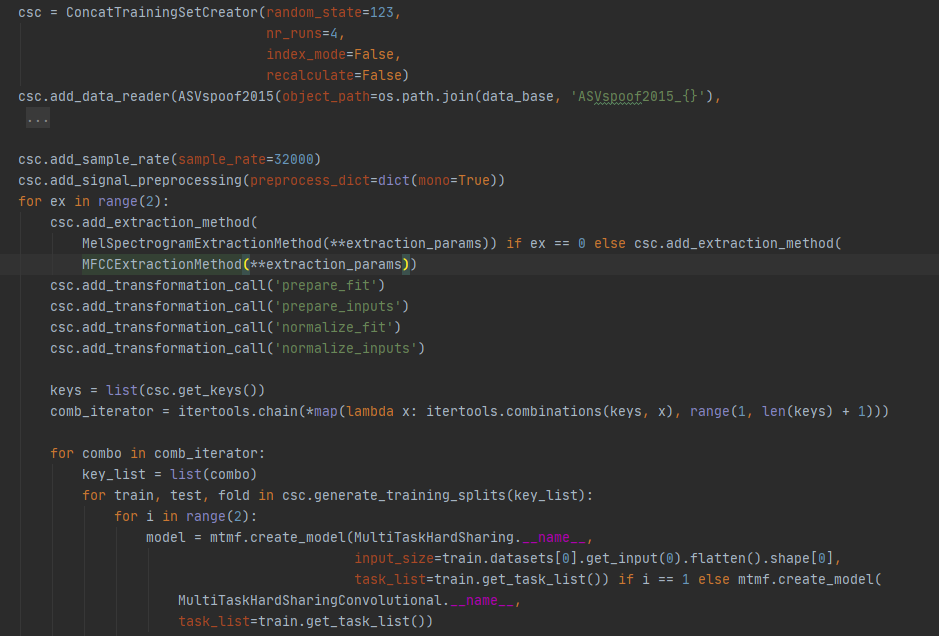
\includegraphics[width=\linewidth]{screenshot005}
	\caption{Data Loading in the variation experiments}
	\label{fig:screenshot005}
\end{figure}

% TODO: Expand on which datasets and what tasks
In total 7 datasets were used in creating this set-up, with 8 tasks. The dataset linked to two tasks is the same used earlier for \citep{georgiev2017low}. The tasks contain both multi-class and multi-label tasks. Each combination is tested for 2 extraction methods and 2 models. For each run, the feature matrices should be framed in the same size, based on the average feature matrix size and the data normalized. As can be seen in table \ref{table:LOC}, this is the first time the required Training LOC makes a significant jump in the Training stage, simply due to the fact that it varies models. The models are loaded for the first time through the MultiTaskModel factory which mainly functions as a way to concentrate static and dynamic model parameters for creation and isn't absolutely necessary. Otherwise, the training is performed using the same three lines as before: model creation, results creation and training loop instantiation. The Data Loading stage also takes a jump, but is in no way related to the high and diverse amount of datasets, simply the variation of elements in the pipeline. There are  operations performed in the pipeline: resampling, conversion to mono, calculating and framing the feature matrices, normalizing the data. The Data loading code can be found in figure \ref{fig:screenshot005}, which makes it apparent that the extra lines outside the transformation calls are simply due to iterating over the required variations. The actual amount of LOC relating to direct data loading operations is 8.\\

This example makes it clear that all the work concerning datasets comes beforehand in the Data Reading stage, with little extra effort on the developer's side, while the combinatorial aspects are handled by the framework in the background. Nothing has to be explicitly reloaded or recalculated, as seen when adding the ExtractionMethod, by the developer as variations will be handled by the framework and necessary data recalculated when required. The framework thus reduces research variations to singular line changes.\\

To build on the last point of reducing work for research variations, especially in future work, it should be noted that given that the previous implementations would have been made as was the case in this scenario, only two extra datasets were added: FSD Kaggle 2018 \cite{fonseca2017freesound} and the Speech Commands dataset  \cite{warden2018speech}. Given that, the Data Reading would be reduced to 8 + 83 LOC in this implementation. DataReader objects are merely paths for extracting the data, while the specifics of how can be given later. Vanilla implementations would either require large code changes if e.g. other extraction methods or signal preprocessing functions were required or have to take these in account beforehand and likely end up with similar structures. \\


\begin{figure}
	\centering
	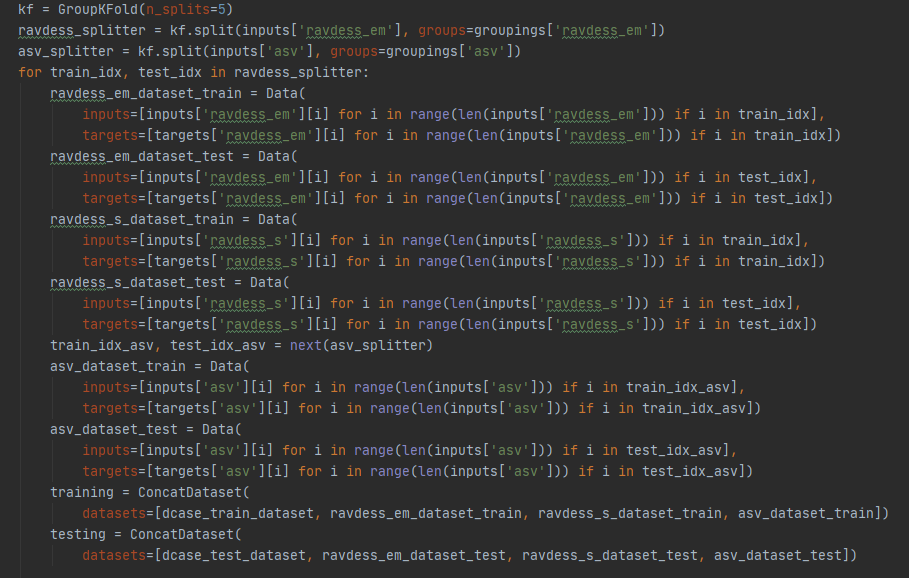
\includegraphics[width=\linewidth]{screenshot002}
	\caption{Train and Test set creation without framework for the \cite{georgiev2017low} implementation}
	\label{fig:screenshot002}
\end{figure}

\begin{figure}
	\centering
	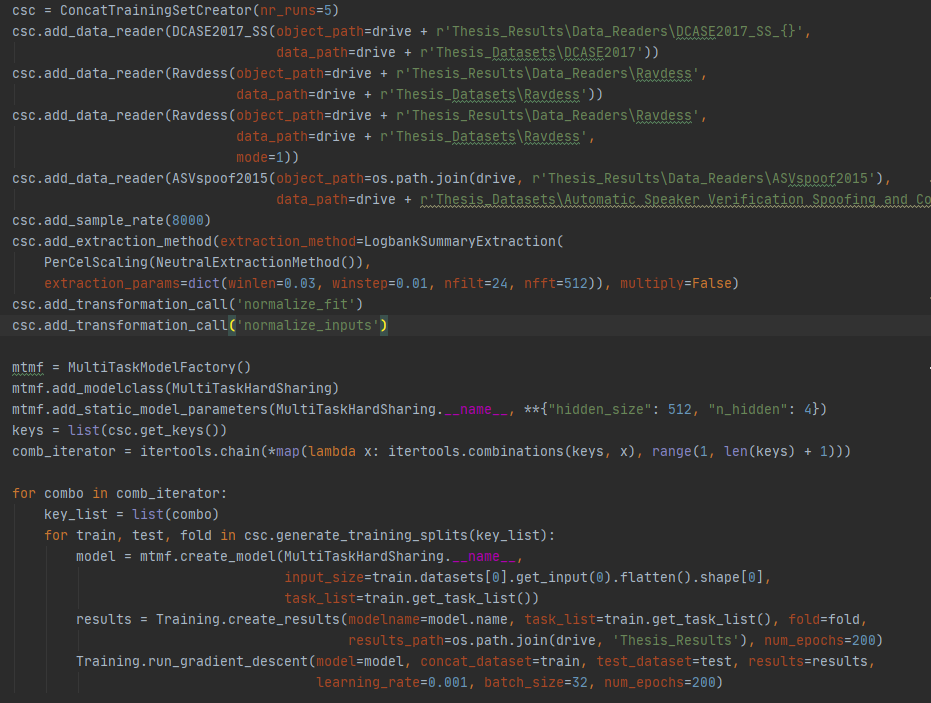
\includegraphics[width=\linewidth]{screenshot003}
	\caption{Complete implementation of \cite{georgiev2017low} with the framework}
	\label{fig:screenshot003}
\end{figure}

What these efforts demonstrate is that the LOC only directly scale with added required operations and do not spill over in other stages. To clarify the last part, figures \ref{fig:screenshot002} illustrate how without the framework, train and test set generation - which falls under the data loading stage - scales directly depending on the amount of datasets used. Compare that to figure \ref{fig:screenshot003}, where it can be seen that train and test generation is actually reduced to one simple line before the three Training stage lines in the end. This also demonstrates how the framework grants flexibility in which datasets to actually load and split with the key\_list input, which grants further work reduction as in practice it is possible that not all datasets are required which were planned beforehand. In the first case, that would imply multiple lines of code change, while in the second, simply one line for the key list. \\

What should again be noted, is that the implementations without the framework did not include a lot of the extra features that are performed automatically, the main one being quick reading and writing of the data. To reiterate, this means that when the Data Reading stage is done, it is written to files on the disk, so that future runs would not unnecessarily have to reextract feature matrices. Including these would raise the LOC required for the vanilla implementations a lot and would either have specific implementations per dataset or end up constructing similar functions to the framework. These LOC comparisons are for the bare required necessities only.\\



%\begin{table}[ht]
%	\caption{Reported metric comparisons} % title of Table
%	\centering % used for centering table
%	\begin{tabular}{p{0.25\textwidth}p{0.25\textwidth}p{0.25\textwidth}p{0.25\textwidth}} % centered columns (4 columns)
%		\hline\hline %inserts double horizontal lines
%		Title & Metric & Reported & Implementation  \\ [0.5ex] % inserts table
%		%heading
%		\hline % inserts single horizontal line
%		\citet{park2020augmenting} & Precision & 0.796 & 0.7741 \\ \hline
%		\citet{park2020augmenting} & Recall & 0.804 & 0.763  \\ \hline
%		\citet{park2020augmenting} & F1 Score & 0.8 & 0.7685 \\ \hline
%		\citet{xu2019multi} & Unweighted Average Recall & 0.662 & 0.6716 \\ \hline
%	\end{tabular}
%	\label{table:metric} % is used to refer this table in the text
%\end{table}
%
%Following the example from other deep learning frameworks like \cite{colacco2020drecpy} it is important that the framework demonstrates to be consistent with published results. In table \ref{table:metric} the comparative results can be found with the original publications. The decision was made to focus on the best reported performance of the multi-task setting, in order to limit the amount of work time to reproduce some of the results. Papers are often incomplete when it comes to specifics required to reproduce the same elements which can impact the results considerably, which requires careful variation and evaluation of the parameters.\\
%
%Starting from the top, the results from the classifier built in \cite{park2020augmenting} come close but slightly below the reports. Multiple node amounts in the DNN were tried, as the original paper lacked to include the exact after the initial layer, yet implying the amount lessen through the figure included. Furthermore, the exact included instances are not the same. The work mentions some cleaning of the dataset was performed, but neglect to mention the specifics. The result is the best performing variation. The amount of nodes was halved in the final two layers and minimal logical clean up was performed (e.g. an audio fragment can not have both silence and another label at the same time). Still, the eventual results end up relatively close to the report.\\
%
%???????????????????????

%Toon in use case met experiment hoe ge een variatie kunt maken aan 1 element in de pijplijn, terwijl de rest intact blijft
%\section{Experiment use case}
%
%%- Describe the goal of making a huge functioning multi-task network
%% Describe the steps of iterative design, demonstrating how single line changes can be made while keeping the rest of the pipeline intact
%% Demonstrate the comparative capabilities in tensorboard
%% Analysis: implementing baseline 
%% iterative design of classifier
%% variation of meta parameters
%% 
%% architecture
%% design
%% construction
%% testing
%% deployment
%% maintenance
%%- Testing different variations
%%- finding the meta parameters
%% comparing to baseline
%
%
%
%
%
%
%Additional to the paper implementations, is an example case study which has been referred to multiple times in this work. The goal is to present how the framework aids the development of multi-task systems by conducting a development process. As stated in \cite{brown1996framework}, this form of evalution is "intended to reveal the broader charactersistics of a technology when it is applied to a representative “complete” problem in an application domain". This case study involves developing a multi-task, multi-dataset neural network which contain a few criteria: \\
%
%\begin{itemize}
%	\item There must be one task that is shared among multiple datasets
%	\item The individual accuracies must reach at least xxx
%	\item The system must be compared to a pre-trained baseline model
%	\item Multiple task types must be present in the combined sets
%	\item The individual performances must be compared to the Multi-Task model outputs
%	\item An extra dataset must be added after completion to test and then expand the training data
%\end{itemize}

%Gender detection in ravdess, asvspoof and chen



\section{Literature Evaluation} \label{evaluation:literature}

%TODO: Dive in the literature and describe its implementation on the software, which components can be adjusted or nah

In line with the goal to provide a tool that can spur development of multi-task research, this section will examine the papers identified in tables \ref{table:combinations}, \ref{table:combinations2}, \ref{table:combinations3} in order to evaluate the expressiveness of the framework as well as its limitations. Specifically, the examination will be made in terms of changes that are required to achieve some of the necessary features. The feature analysis of the framework is performed by analysing the papers as problem contexts for identifying model problems \citep{brown1996framework}. The goal is to identify possible limitations to the architecture and possible future extensions that are required. \\

To do this, an examination of specific techniques that are present in the literature is made and discussed to what degree and facility they can be implemented by the system. Mainly techniques that haven't been clearly been addressed in previous sections, but have presence in the literature are brought up here. From this, conclusions are drawn towards what future development can focus on to provide a more complete framework for multi-task development and what the limitations are of the (current) design.\\


% - Multichannel feature extraction available by input
% - Signal processing scaling: data augmentation

\underline{\textbf{Input Techniques.}} The first set of techniques are related to input requirements. The framework's data structure for encapsulating inputs is a list of tensors that are, by index, related to one or multiple targets. Each input can either be added directly as a tensor or as a signal from which the feature matrix is extracted on input using the TaskDataset's ExtractionMethod object. In any case, once the data is encapsulated within the TaskDataset, it is always a feature matrix which is ready to serve as input for the training function. There are (limited) functionalities available for transforming audio signals before extraction through the DataReader's process\_signal function.\\

While most research utilize \textbf{mono channel} audio signals \cite{seltzer2013multi} \cite{panchapagesan2016multi} \cite{kim2017speech}, there are instances where \textbf{multi-channel signals} are used, even as much as four \cite{nwe2017convolutional}. The framework's extraction methodology already takes this situation into account, creating parallel feature matrices and concatenating them into a singular input instance. In some instances though, stereo input signals are transformed to mono channel signals in order to reduce the feature matrix size. This situation is already covered as well as part of the process\_signal function, where a multi-channel signal is averaged to a single channel at the command of an input boolean, meaning it can varied at runtime.\\

However, this brings up the way \textbf{signal processing} is handled in the framework. Its limitations become apparent when more signal transformations need to be performed. For example the data augmentations described in \cite{lopez2019keyword} would be a problem in the current setting. In this scenario, multiple randomized signal transformations are applied to a single fragment, before MFCC features are extracted. In order to scale this operation for multiple datasets, the developer has two options. One is to create an extension to the DataReader class which are in turn extended by each of their DataReaders for the individual datasets. The other is to store the signal as a tensor and encapsulate the data augmentation techniques in the preparation function of the ExtractionMethod class. Sadly, there are complicating factors which do not make the described augmentation method possible, as additional noise segments from random files in their dataset as well as the augmentation being recalculated every epoch for 30\% of the dataset. \\

This case thus highlights two problems in the signal preprocessing approach: it is messy to create extra pre-processing functionalities and it is impossible or very complicated to vary steps in creation of the input between epochs. At first sight, creating a standardized approach for addressing this specific situation would be complicated due to the reliance on an additional dataset for noise fragments. The TaskDataset structures are not designed with access to the original dataset in mind, nor do they currently offer any storage of additional information.\\

% - Multi input form
% - training adaptation: targets as inputs
Moving on to examining what singular \textbf{input instances} actually are. In pretty much all the research, an input instance is a single feature matrix, which is the result of an extraction methodology applied to an audio signal. However, two works challenge this form.\\

The first one is \cite{fernando2020temporarily}, where the \textbf{input for a single audio fragment comes in three forms}: The time series, the MFCC features and the MFCC deltas.  These three representations are combined into a single LSTM encoder which results in the actual input embedding. This embedding is then used along with a random noise vector as an input for a Generative Adverserial Network (GAN). However this network is trained (encoder LSTM trained separately or together with the rest of the Multi-Task network), there is no issue as tensors can be created which are concatenated from matrices with different dimensions. The one caveat however is that, in order to batch multiple instances, the individual tensor dimensions must be equal, but this is always the case anyway, which is why windowing transformations are standard available. The current implementations however only take two dimensional matrices in account. If every instance does have variable shapes, a custom DataLoader must be created, which would be the case anyway without the framework. No extra complications are introduced due to the option to input the DataLoader in the training and evaluation functions.\\

A more difficult situation however is found in \cite{komatsu2020scene}, where \textbf{target labels from one task are served as input} for the additional task. Targets are not given as input for the model in training, which means that these should be included as part of the input matrix. The issues that this causes however are minimal, as it means that target vectors have to be stored twice, which wastes space. \\

These cases impose less severe issues, but do require forms of extraction and forming the classifier in a way which would inhibit easy addition of new datasets. Besides, the models would also have to include steps to split up these concatenated tensors, which possibly introduce too many undesired calculations. More flexibility to deal with these situations could be provided by allowing multiple input instances per fragment, similar to how multiple targets are possible per instance. \\

% - Targets flexibility other than labels
% - self-supervised tasks require ...
% - self-supervised tasks also like adaptation mechanisms
% - Parallel models with one pretrained possible but with some caveats
\underline{\textbf{Target Techniques.}} The next category includes techniques related to how the targets are formed. Targets are assumed to be vectors and are stored as lists of integers. In the current setting, targets are labels which are numeric, either discrete, representing categories or continuous for regression tasks. In short, the targets are made for supervised labeled learning tasks.

Of course this makes the current framework not optimised to store any other \textbf{target structure}. A first example of this comes in \cite{lu2004multitask}. In this work, speech enhancement is implemented as an additional task to improve the automatic speech recognition task. Speech enhancement requires \textbf{clean speech signals as targets} on which a loss function is calculated to measure the discrepancy between noisy and clean signals. Creating an extension to the TaskDataset to allow targets other than labels doesn't sound too complicated. The issue comes when combining multiple taskdatasets.\\

In order to allow for batching operations, which combines instances of targets in a singular matrix. However, in order to allow an unspecified amount of tasks - coming from tasks which may or may not be present within the TaskDataset at hand - target labels are combined within a single target vector, with dummy \textbf{padding for the targets} that are not present. When targets become multidimensional, this structure consequently falls short. This signals a requirement more sophisticated ways to encapsulate multiple instances for input matrices and targets, but has to pay attention not to introduce unnecessary computational complexity for the simpler cases. \\

Mentioned above is the fact that the system is currently based around supervised, labeled learning tasks. \textbf{Self-supervised tasks} like in \cite{lee2019label} are not that much of a problem. As these tasks are based on loss functions which calculate on internal parameters or outputs (e.g. distance metrics), these can be either added in the form of a task object with dummy labels or directly extended in the Training\_Util's loss calculation function. Tasks have to have target labels, which do add small unnecessary extra memory usage. The loss functions themselves can be formed as normal PyTorch loss functions, which means no extra work load is introduced. An extra option is to include it in the model itself.\\

\textbf{Adaptation mechanisms} like the gating mechanism in \cite{tagliasacchi2020multi} are in the same vein as self-supervised tasks. In \cite{tagliasacchi2020multi}, an internal gating mechanism for prediction outputs is created, which adapts based on a cost function of utilising more channels. This cost function is combined with the normal loss calculation and the model is optimized through the regular back propagation method used. Each task has its own cost function calculated, but also can either be implemented within the model itself or added as an extra task with dummy labels.\\

The final case is that presented in \cite{wu2020domain}. The work presents a multi-task model, with two parallel models that in one model uses the output of an internal layer from the parallel classifier. The catch is that the parallel \textbf{classifier is pre-trained}, so its output would not be required to be utilised in updating the multi-task model, nor would its layers be updated. The framework would not even require any extension for this case, as the training set can simply not contain the extra task, but the testing set would. The model creation is entirely modularly separated from the rest of the framework, so different subsections and combinations of the dataset can be used for the model training and evaluation. As long as it arrives in the form of a TaskDataset, the model will be fed (batched) instances.\\


% - One dataset, multiple supervised tasks possible
% - Loss calculation adaptations: weighted loss combinations
% - Loss calculation adaptation: Teacher student model
% - RBM's not possible due to non-gd training
\underline{\textbf{Loss Functions.}} In this part, methodologies concerning loss functions are examined. The current methodology places one loss function per task. These are calculated for each task in each batch separately, after which they are combined. The combined loss is used for the backpropagation update of the network. Both the separate loss calculations and combination of those losses are part of the functions in the Training\_Utils object. Remember that earlier it was stated the training and evaluation loops were designed not to be touched, but the functions included in the Training\_Utils object do offer modification options which can be varied at runtime, by instantiating a different Training\_Utils object. \\

With the current systems in place, the target structure from earlier is assumed and the different tasks' outputs are taken by breaking up the target vectors. Any amount of different supervised is thus not a problem, with the instances of the batch they apply to also being taken care of. The combination simply sums up the losses. The separate calculations and combination of those losses are two separate functions, so a small adaptation like \cite{park2020augmenting} of \textbf{introducing weights} can simply be added in that extension. Loss functions, contained in the Task objects, are given at instantiation and can be varied at runtime.\\

This structure of doing things, does however require the implementations of those functions to work with what was received in the training loop. Neither receive the input feature matrices. This can be limiting to \textbf{teacher student training models} like in \cite{imoto2020sound}. This methodology is similar to the parallel models in \cite{wu2020domain}, except that the parallel model is only used in the training phase as a way to train one of the task heads. The loss is not calculated on predefined ground truth labels but labels outputted in the parallel pre-trained model. This is only a problem however if the parallel model's outputs have to be calculated at runtime for some reason however, in stead of pre-predicting the instances and storing them as normal targets in a TaskDataset. \\

Finally, it has been mentioned often, but the training loop is only targeted at \textbf{gradient descent} based training, following PyTorch's methodology for performing these. However, forms of training that can not be written this way would require their own training implementation. This also limits some forms of NN to utilize the current training loop. In \cite{georgiev2017heterogeneous} for example, a RBM network is additionally created which requires greedy layer wise pre-training, which would not be possible through the framework.\\

\cite{georgiev2017heterogeneous} also shows the last technique which would not be possible in the current state, which is \textbf{mini-batch SGD}. There is a reason the training loop function is called run\_gradient\_descent as it does implement a standard gradient descent loop. In many ways this also illustrates why the choice was made to require the developer to make their own implementation of the training loop. The loop consists of the standard gradient descent training loop which elements can be individually interchanged. Other training procedures could be and possibly bloated to create standardized solutions for, while the developer can still utilize the same building blocks that offer its variability qualities.\\

\underline{\textbf{Conclusions}}

% Inputs:
% - Signal processing's scalability can be higher
% - Multiple matrices for one instance should be considered
% None of these are insurmountable, but would off better functionalities and streamline its use
After examining the literature, some conclusions can be drawn regarding what the framework lacks or can be improved in. In general, the main limiting factors regarding the optimal implementation of research methodologies can be found in the data structures for encapsulating the inputs and targets and the rigid structure of the training mechanism. \\

The signal pre-processing, which happens in the DataReader classes, by utilizing their shared preprocessing function could use a more scalable, extendible format. Currently either a new extension to the DataReader class has to be made. Furthermore, the addition of allowing multiple feature matrices for one data instance should be considered. These input related issues do not prohibit any implementation to be made but do require circuitous solutions due to the framework.\\


% Targets
% - Requires more flexible forms of targets. For that the combining methodology must be reworked.
% - Loss functions/Tasks without targets should become possible
In the target structures are more severe issues for implementing certain techniques. Allowing other target forms from labels are crucial for certain tasks even within supervised learning problems. This in turn would also require the way the system combines targets for batching to change from the padding that currently. Less severe is that tasks with loss functions should become possible without targets which would allow for more straight forward multi-task implementations which optimize for non label based loss functions as well, but there are workarounds as discussed.\\

% Loss functions
% - 
In the sense of the training function, the rigid structure which requires the developers own implementation if changes are required that can not be achieved by extending the Training\_Utils class. Adding small elements like mini-batching requires rewriting the training algorithm completely. Also does the training mechanism only function for gradient descent based training. \\



% General:
% More open training mechanism:
% - augmentation every epoch case
% - control over input for model -> target labels as input case



% 



% Make table with things that require big changes (i.e. the core)
% Make a table with things that require extensions
% Make a table that overviews the possible/not possible




\section{Fulfilment of the Requirements}

This section contains a point by point discussion of the designated functional and non-functional requirements

\subsection{Non-functional Requirements}
\begin{itemize}
	\item \textbf{Modular:} 
	%	Demonstrate the replaceability in the code
	The framework is largely modular as a central design point. The framework presents developers with the loose tools to design and implement a multi-task pipeline at different levels. The DataReader gives a loose structure to extract a dataset's inputs, targets and additional task information. The DataReader's open design merely gives a common structure and tools to create a TaskDataset, as well as implement the quick reading mechanism, yet has no obligation to output a TaskDataset object. The TaskDataset and related structures offer a unified way to encapsulate the extracted dataset. The training and evaluation loop offer the ability to load batches of inputs and targets from a PyTorch Dataset, utilise them to predict the outcome using the neural network. To compose the pipeline, the TrainingSetCreator structure is in place, which creates the path from the raw datasets to the processed and transformed inputs for the training and evaluation mechanisms. The TaskDataset's use in the taining mechanisms and the TrainingSetCreator is not a full on dependency but does require specific requirements for an alternative to be met. For the Training and Evaluation mechanism, this is nothing more than the fact that an input and target batch are outputted in tuple form when getting an individual instance. If so, then it doesn't matter what type of Pytorch's Dataset is given as its input. The TrainingSetCreator however does utilise the added functions of the TaskDataset and the HoldTaskDataset. While this does add a dependency on the TaskDataset structure, the different phases - Data Reading, Data Loading and Training - are still completely independent from each other. Whithin each of those phases, there are numerous different elements that have been shown to be easily variable either at implementation level or at runtime, depending of the necessity. \\
	\item \textbf{Extendible:} 
	%	Extensibility is discussed in design section
	The design's extensibility is discussed in its own implementation section \ref{Impl:Extendibility}. The framework builds atop of PyTorch's basics for the static data structures, which mimics its own extensibility. Every implementing class has constraints which would ensure its applicability in the rest of the system in case a developer needs to develop an extending implementation. The non-static datastructures, which refer to functions like the training loop and the TrainingSetCreator, make sure to keep its dependencies on a function basis, meaning that every function deals with one type of data structure and thus only those functions need to be extended. 
	
	The Framework's extensibility is mostly open due to its modularity. As the few requirements for the usage of objects in other classes are met, every functionality and more can be changed or added. Mainly the training and evaluation functions are defined pretty rigidly in the sense that they have to be completely reimplemented in certain cases. Otherwise, the extraction methods, the data transformations, the tasks, the loss functions and many more described above can be extended and introduced, without having to touch any other part of the framework. Section \ref{evaluation:literature} offers insight to the limits of the extensibility compared to the requirements that were posed in the literature. Especially the transformations of Datasets are completely open for extensibility even with the TrainingSetCreator, as they are called through their naming convention.\\
	
	\item \textbf{Fast prototyping:} 
	% Demonstration implementations, comparison with implementation without
	The speed of prototyping is achieved in two ways in the framework. The first is presented in section \ref{evaluation:demonstrations}, where it shows how a lot of papers' described methodologies can be shortened through usage of the system's functions. The second lies in the system's TrainingSetCreator structure, which automatically will form defined dataset pipelines and recalculate them if new parts are introduced. When fine tuning a new system, the developer can thus change variables and functionalities while the TrainingSetCreator will now what parts to recalculate on the fly. This way, both set implementations as well as iteratively designed and fine-tuned implementations of networks have reduced work loads. 
	\item \textbf{Cutting Double Work:} 
	% Demonstration of the research set-up
%	\item \textbf{Developmental Side-rails:}
%	%  
	In section \ref{evaluation:demonstrations} as well as the previous item, it is discussed how the framework handles pipelines to avoid double recalculations, with section \ref{evaluation:literature} discussing it limits. However, finding the right meta-parameters and optimizing the process steps get cut through the TrainingSetCreator's management of pipeline parts. Furthermore, the quick reading functionality standardly offered through the DataReader prevents unnecessary recalculation of features which can take up a lot of computational resources.  
	\item \textbf{Flexible:} 
%	Demonstration + Dive in the literature
	The flexibility as well as its limits have been thoroughly discussed in secion \ref{evaluation:literature} and the previous chapters. To summarize, the framework optimizes for numerous supervised learning cases, but still has some blind spots, especially for non-supervised training set-ups. When the data is encapsulated as a TaskDataset, the training and evaluation loops will have no trouble processing regardless of what it encapsulates.
\end{itemize}

\subsection{Funtional Requirements}
\subsubsection{Data Reading}
\begin{itemize}
	\item Standardizing Input - The TaskDataset object is developed for assuring that the data is valid throughout the rest of the process. Its extension of PyTorch's Dataset class ensures that it can be utilised by the PyTorch framework. The builder pattern allows the TaskDataset to be built incrementally and valid along the way, with each step including various validity checks.
	The exception where the TaskDataset can't check for validity is in terms of the input feature matrix size. The matrix sizes might not be compatible with the developed PyTorch Model. The responsibility for this is up to the developer.
	% How do we know this works?
	% What validity checks?
	\item Handling dataset differences - The DataReader class is an abstract class that the developer must extend to deal with the peculiarities of navigating each dataset structure to extract the correct information. This corresponds to it being a white box hot-spot. Predefined train/test splits can be stored through the HoldTaskDataset structure and pre-split audio segments can be kept together by defining the grouping. 
	% Refer to the implementations for differences
	\item Scalable preprocessing - Preprocessing audio signals and preprocessing feature matrices happen in different places, as TaskDatasets should only contain valid input instances at any point. Preprocessing signals can utilise an (optional) function from the DataReader class with parameters that are received when the TaskDataset is extracted. Reusing the method can thus hand developers easy replicability of the signal preprocessing. These can be further scaled by using the TrainingSetCreator. In this class, any preprocessing or transformation can be added 'on the fly'. This means that if a functionality (e.g. resampling) is added, any previous 
	% What preprocessing do we have for both signals and feature matrices
	\item File storage abstraction: There are handles on the TaskDataset which can be called to store, load or check the TaskDataset to or from files, which are specific for the currently used extraction method and task.
	\item Quick Reading: The DataReader automatically checks if there is a stored TaskDataset available for the given extraction\_method and task and loads it if so.
	\item Create multiple input objects from the same dataset: The framework is open ended in how the TaskDataset object is extracted from the data and allows extra parameters for the DataReader to be given at initialization. TaskDatasets are stored using the ExtractionMethod object's name and the (main) Task's name, so for every new variation of these will be automatically linked to different files.
	\item Tasks and datasets are a many to many relationship: Tasks can be present in multiple datasets. The tasks need to have the same name, output labels and classification type in order to be seen as the same. When combined in the ConcatTaskDataset, the target vectors will automatically be placed in the same positions, which will make them be seen as the same task in the training function. Datasets can have multiple tasks to an unlimited degree in its list of extra tasks, which always combines them with a list of targets of the same amount of input instances. 
\end{itemize}
\subsubsection{Data Loading}
\begin{itemize}
	\item Combining datasets: The ConcatTaskDataset can hold and present multiple datasets as a single bigger dataset, while helper functions allow multiple data instances to be batched. Furthermore, a data loader is provided which can randomly load batches from alternating tasks, which would forego the need to have a unified matrix size across tasks. The loss calculation present in the training and evaluation functions automatically pick apart the prediction outputs and only use the correct data for the related task's loss function. 
%	Extended the ConcatTaskDataset, extra functions for the batching
	\item Not requiring the combined datasets in memory:  Index mode implemented which forms a streaming context for the data to be stored and read from disk. The index mode can be automatically given as a parameter for initializing a TaskDataset, which makes it very easy to switch to. The more datasets are added, the more likely this scenario is, so a runtime switch between holding the data in memory or reading it from disk can both permit implementations to be executed and cut complicated redevelopment work.
	\item Train and test set generation: The HoldTaskDataset is responsible for all train and test set generation functionalities added to a regular TaskDataset. TaskDataset functions can be called which will automatically be called accordingly on the Test set as well. The TrainingSetCreator can also be called which operates the training set generation and functions called to refine the TaskDataset in the correct order. Furthermore, there is support for k-fold validation in both these classes as well. Every new fold generated also rewinds normalizations which were based on training set metrics.
	\item Transforming data: There are two functions present in the TaskDataset for transforming the data, one for scaling the input instances and one for further transformations like cutting the matrices into same sized frames. Both of these operations are implemented on an instance basis in the ExtractionMethod object given to the TaskDataset. The functions on the TaskDataset themselves simply call these to transform every individual input matrix. The TrainingSetCreator can dynamically add new transformations through the add\_transformation function, which operates based on names, making it open to extended implementations of the TaskDataset that have more functions. Also available is multiple TaskDatasets sharing the same ExtractionMethods, which would let them share the same metric calculations and thus perform the same transformations as if they were one unified dataset. The TrainingSetCreator can do this automatically at the command of one boolean at input. This is also the reason that the transformation and their calculation functions work instance based in stead of the whole dataset at once.
%	They implemented through handles on the TaskDataset which call upon the ExtractionMethod
	\item Filtering data: Data can be filtered through the sample labels function present on the TaskDataset. The developer can even use this to change the task itself by removing all instances with a specified label and remove its mention in the Task object automatically.
%	Handle on the TaskDataset
	\item Reusing data: The TrainingSetCreator is the class which manages the multi-dataset pipeline. Here, the DataReaders are given as input, while steps in the pipeline (e.g. pre-processing, filtering, transformation,...) can be dynamically added to one specific or all datasets. Only when the dataset creation function is called, do the actual TaskDatasets get created and stored. However, if any step is replaced after creation, the TrainingSetCreator will only reload or recalculate the affected dataset. To minimize unnecessary data usage, which exact present TaskDatasets get created can be determined by the developer, while all other unnecessary TaskDatasets get removed from memory.
%	It implemented, reusability is possible without reloading to different degrees
	\item Batching multiple tasks: Multiple tasks can be combined in multiple datasets. As mentioned before tasks and datasets are many-to-many relationships and the tricky issue is to fit a variable amount of tasks, connected target labels and the fact that tasks can be present in multiple TaskDatasets in batches which could include instances from any dataset. Therefore the padding system was developed which also has its limitations concerning targets that are not labels as identified in section \ref{evaluation:literature}.
%	It implemented lol
	\item Replicability: Extraction method objects are stored, including their calculations in order to recreate the extraction and the subsequent transformations. Beyond that, the system's randomness based functions like filtering make sure to include optional keys for pseudo random number generation to replicate the same pipelines as previous runs. The training mechanism also stores the model's state at every epoch, through the Results object. Recreating a Results object with the same name, pointing at the same folder location gives automated access for reloading old checkpoints and written metrics. Even more is the fact that the evaluation function further automates this system by including the opportunity to insert a blank model, which in cooperation with the Results object would load and evaluate these old models for all or a subset of the epochs.
%	It implemented through storing the different checkpoints (which can be recreated by reloading the Results object), the calculation data in extractionmethods and 
	\item Scalable Manipulation: In the TrainingSetCreator, manipulations can be added for one specified dataset or all at once. These manipulations do not only include the TaskDataset's methods, but also pre-processing parameters and ExtractionMethod objects, which can be replaced at runtime.
\end{itemize}
\subsubsection{Training}
\begin{itemize}
	\item Predicting multiple tasks: Each dataset can have multiple tasks linked to their targets. There are automatic filters for the output to isolate the task specific predictions. 
	\item Task specific output handling: Handling of the task functions, like loss calculation and decision making of the eventual classes from the probabilities are stored in the Task objects 
	\item Loss calculation specifiable: The calculation of the Loss of each task is definable in the Task object. However, currently, losses are always tied to tasks, which have target labels. This is not always the case, as in the research \citep{tagliasacchi2020multi} \citep{wu2020domain}, losses have also been calculated based on cost functions from internal model parameters. Since these loss functions are not linked to datasets, but to the models themselves, for which the framework does not offer modules which can be used in the training function for specific handling, it is up to the developer to implement these in the Training\_Utils object.
	\item Loss combination specifiable: Implemented in the Training\_Utils object
	\item Metric calculation, storage and visualization: Gives predictions, true labels and losses to the Results object which calculates the metrics, stores them and writes them to tensorboard where they can easily be compared to other results
	\item Interrupted Learning: (DEMONSTRATE) Implemented by recreating the Results object and starting the training loop from the given epoch.
	\item Separate evaluation: (DEMONSTRATE) The evaluation function is separate from the training loop. Training parameters for transformations and such can be reloaded from the stored extraction\_method object as well as the model parameters at every epoch in the training function. 
	\item Direct comparison of different runs: Every run has a unique name and TensorBoard has the ability to place the results from different files side-by-side
	\item Variable training paradigms: In this state, the only training paradigm available is Gradient Descent. Implementing a different paradigm requires foregoing the current training loop implementation.
\end{itemize}